\section{Konzeption und Umsetzung}
\label{sec:4}
\subsection{Idee}
\label{sec:4.1}

Da die Ergebnisse dieser Arbeit relevant für das KoViTReK Forschungsprojekt\footnote{\url{https://www.th-koeln.de/anlagen-energie-und-maschinensysteme/kovitrek\_87259.php}}
sein könnten und dieses in der Laufzeit- und Entwicklungsumgebung Unity\footnote{\url{https://unity.com}}
implementiert werden soll, werden auch die Partikelsysteme in der selben Umgebung entworfen.

Ein wichtiger Faktor bei der Darstellung von Rauch ist die Beleuchtung. Eigenschaften wie Streuungen und Reflexionen innerhalb des Mediums zu simulieren ist
aufwändig zu berechnen und bisher nicht für die Echtzeitberechung in VR-Systemen, welche deutlich höhere Anforderungen an die Performance der Anwendung
haben, gedacht.
Der erste Ansatz basiert auf einer Idee von Mederic Chasse, Technical Art Director  bei Highwire Games.
Dieser schlägt einen Workflow vor, mit dem aufwändige Berechnungen solcher Simulationen in einer VFX Software erstellt, berechnet und gerendert werden.
Die Animation wird in einem Texture Sheet gespeichert und kann somit den Einsatz in einer Game Engine sehr effizient machen und eine realistische Darstellung bieten \parencite{Chasse2018}.
Da der Fokus dieser Arbeit nicht auf der Fluidsimulation liegt und das Setup der Simulation mithilfe von Anleitungen
und Tipps artistischer Natur aus Internetforen erzeugt wird, wird an dieser Stelle nicht weiter darauf eingegangen, wie die VFX-Software den Rauch berechnet und erzeugt.
Stattdessen wird in \textbf{\autoref{sec:4.2.1}} der Workflow beschrieben und auf einige Parameter der Simulation eingegangen.

Für die Darstellung mithilfe von Ray Marching werden richtige Volumendaten, bzw. 3D-Texturen benötigt. Diese werden innerhalb von Unity
mithilfe eines Shaders prozedural erzeugt. tba


\subsection{Erstellung der Texturen}
\label{sec:4.2}


\subsubsection{Texture Sheets}
\label{sec:4.2.1}
\begin{figure}[h!]
	\includegraphics[width=0.49\textwidth]{Grafiken/Implementation/Lightmaps/Smoke_LightSetup.png}
	\centering
	\begin{footnotesize}
		\caption{Setup der Beleuchtung der Rauchsimulation in Houdini.}
		\label{fig:lightSetup}
	\end{footnotesize}
\end{figure}

Die Texturen werden auf zwei verschiedene Arten erstellt. Für die Variante mit Parallax Occlusion Mapping werden zwei
Texturen in der von SideFX entwickelten 3D-VFX-Grafiksoftware Houdini \footnote{\url{https://www.sidefx.com/products/houdini/}} erstellt.
Houdini bietet die Möglichkeit relativ einfach und schnell physikalisch basierte und visuell überzeugende Rauch- und Feuersimulationen zu erstellen.
Die Simulationen basieren auf Fluidberechnungen, wodurch ein realistisches Verhalten erzeugt und durch eine Vielzahl an Parametern beeinflusst werden kann.

Hier noch kurz die wichtigsten Parameter beschreiben, zb. Buoyancy, Dichte, Short tail des Rauchs, damit dieser eher aussieht wie ein Rauchball

Dabei wird nicht nur die Beleuchtung der Oberfläche aus verschiedenen Richtungen, sondern auch die Streuung, Reflexion und Absorption des Lichts innerhalb
des Volumens berechnet und simuliert.
Eine Möglichkeit die Houdini bietet, ist das Rendering der Animation in verschiedene Layers. So kann jedes einzelne Licht separat berechnet, gerendert und
hinterher separat verwendet werden. Dazu werden Lichtquellen wie in \textbf{\autoref{fig:lightSetup}} aus allen sechs Richungen zum Rauch hin angeordnet,
sodass jeweils eine Seite beleuchtet wird.
Die Animation des Rauchs wird daraufhin wie in \textbf{\autoref{fig:seamlessCut}} in eine sich selbst nahtlos wiederholende Animation
geschnitten und als einzelne Frames gerendert. Dazu muss im ersten Schritt eine Animation mit der doppelten Anzahl an Frames erzeugt werden, damit diese in der Hälfte
geschnitten werden kann. Nun werden die beiden Abschnitte übereinander gelegt, sodass sich die Schnittkante auf gegenüberliegenden Seiten befinden. Somit sind der erste
und der letzte Frame nahezu identisch. Als letztes wird ein Crossfade über beide Abschnitte gelegt, sodass die Clips jeweils an der Schnittkante voll eingeblendet
sind. Somit ist der Schnitt nicht mehr sichtbar und das Video lässt sich unendlich wiederholen. Die Vorteile von dieser Methode werden in \textbf{\autoref{sec:5.1}}
noch weiter erläutert.
Um die verschiedenen Texturlayer in Unity verwenden zu können werden die Lichtrichtungen jedes einzelnen Frames in jeweils einen RGBA-Channel gelegt.
So kann die Ansicht des Rauchs, in der beispielsweise nur die linke Seite beleuchtet wird in den Roten Kanal einer Textur gespeichert werden.
Dies passiert ebenfalls für die anderen Richtungen von links, unten und oben. Die Ergebnisse sind in \textbf{\autoref{fig:lightDirections}} zu sehen.



\begin{figure}[h!]
	\includegraphics[width=\textwidth]{Grafiken/Implementation/Lightmaps/SeamlessCut.png}
	\centering
	\begin{footnotesize}
		\caption{Schritte um Loop einer Rauchanimation ohne sichtbaren Schnitt zu erzeugen. }
		\label{fig:seamlessCut}
	\end{footnotesize}
\end{figure}

\begin{figure}[h!]
	\centering
	\includegraphics[width=0.19\textwidth]{Grafiken/Implementation/Lightmaps/T1_R.png}
	\includegraphics[width=0.19\textwidth]{Grafiken/Implementation/Lightmaps/T1_G.png}
	\includegraphics[width=0.19\textwidth]{Grafiken/Implementation/Lightmaps/T1_B.png}
	\includegraphics[width=0.19\textwidth]{Grafiken/Implementation/Lightmaps/T1_A.png}
	\includegraphics[width=0.19\textwidth]{Grafiken/Implementation/Lightmaps/merged.png}

	\begin{footnotesize}
		\caption{Ein einzelner Frame der Simulation in seine Farbkanäle aufgeteilt. Die Richtungen aus denen der Rauch jeweils beleuchtet wurde ist dabei gut zu erkennen.
			Von links: Roter Kanal(links), Grüner Kanal(rechts), Blauer Kanal(oben), Alpha Kanal(unten), Zusammengeführte Textur.}
		\label{fig:lightDirections}
	\end{footnotesize}
\end{figure}


Die verschiedenen Farbkanäle können nun wieder in eine gemeinsame Textur zusammengeführt werden um dann in Unity in einem Shader weiterverarbeitet zu werden.
Dabei wird jeder Frame mit einer Auflösung von 128x128 Pixel gespeichert. Bei einer Frameanzahl von 8x8 = 64 Frames entspricht das also
einer Auflösung der ganzen Textur von 1024 x 1024 Pixel.

Damit Parallax Occlusion Mapping angewendet werden kann werden jedoch zusätzlich Informationen über die Höhe benötigt.
Dazu wird eine zweite Textur mit den gleichen Schritten wie zuvor erzeugt. Neben der Höheninformation wird außerdem noch die Alpha-Werte, sowie zwei weitere Lichtrichtungen –
von vorne und von hinten – in die verschiedenen Kanäle gespeichert.




\begin{figure}[h!]
	\centering
	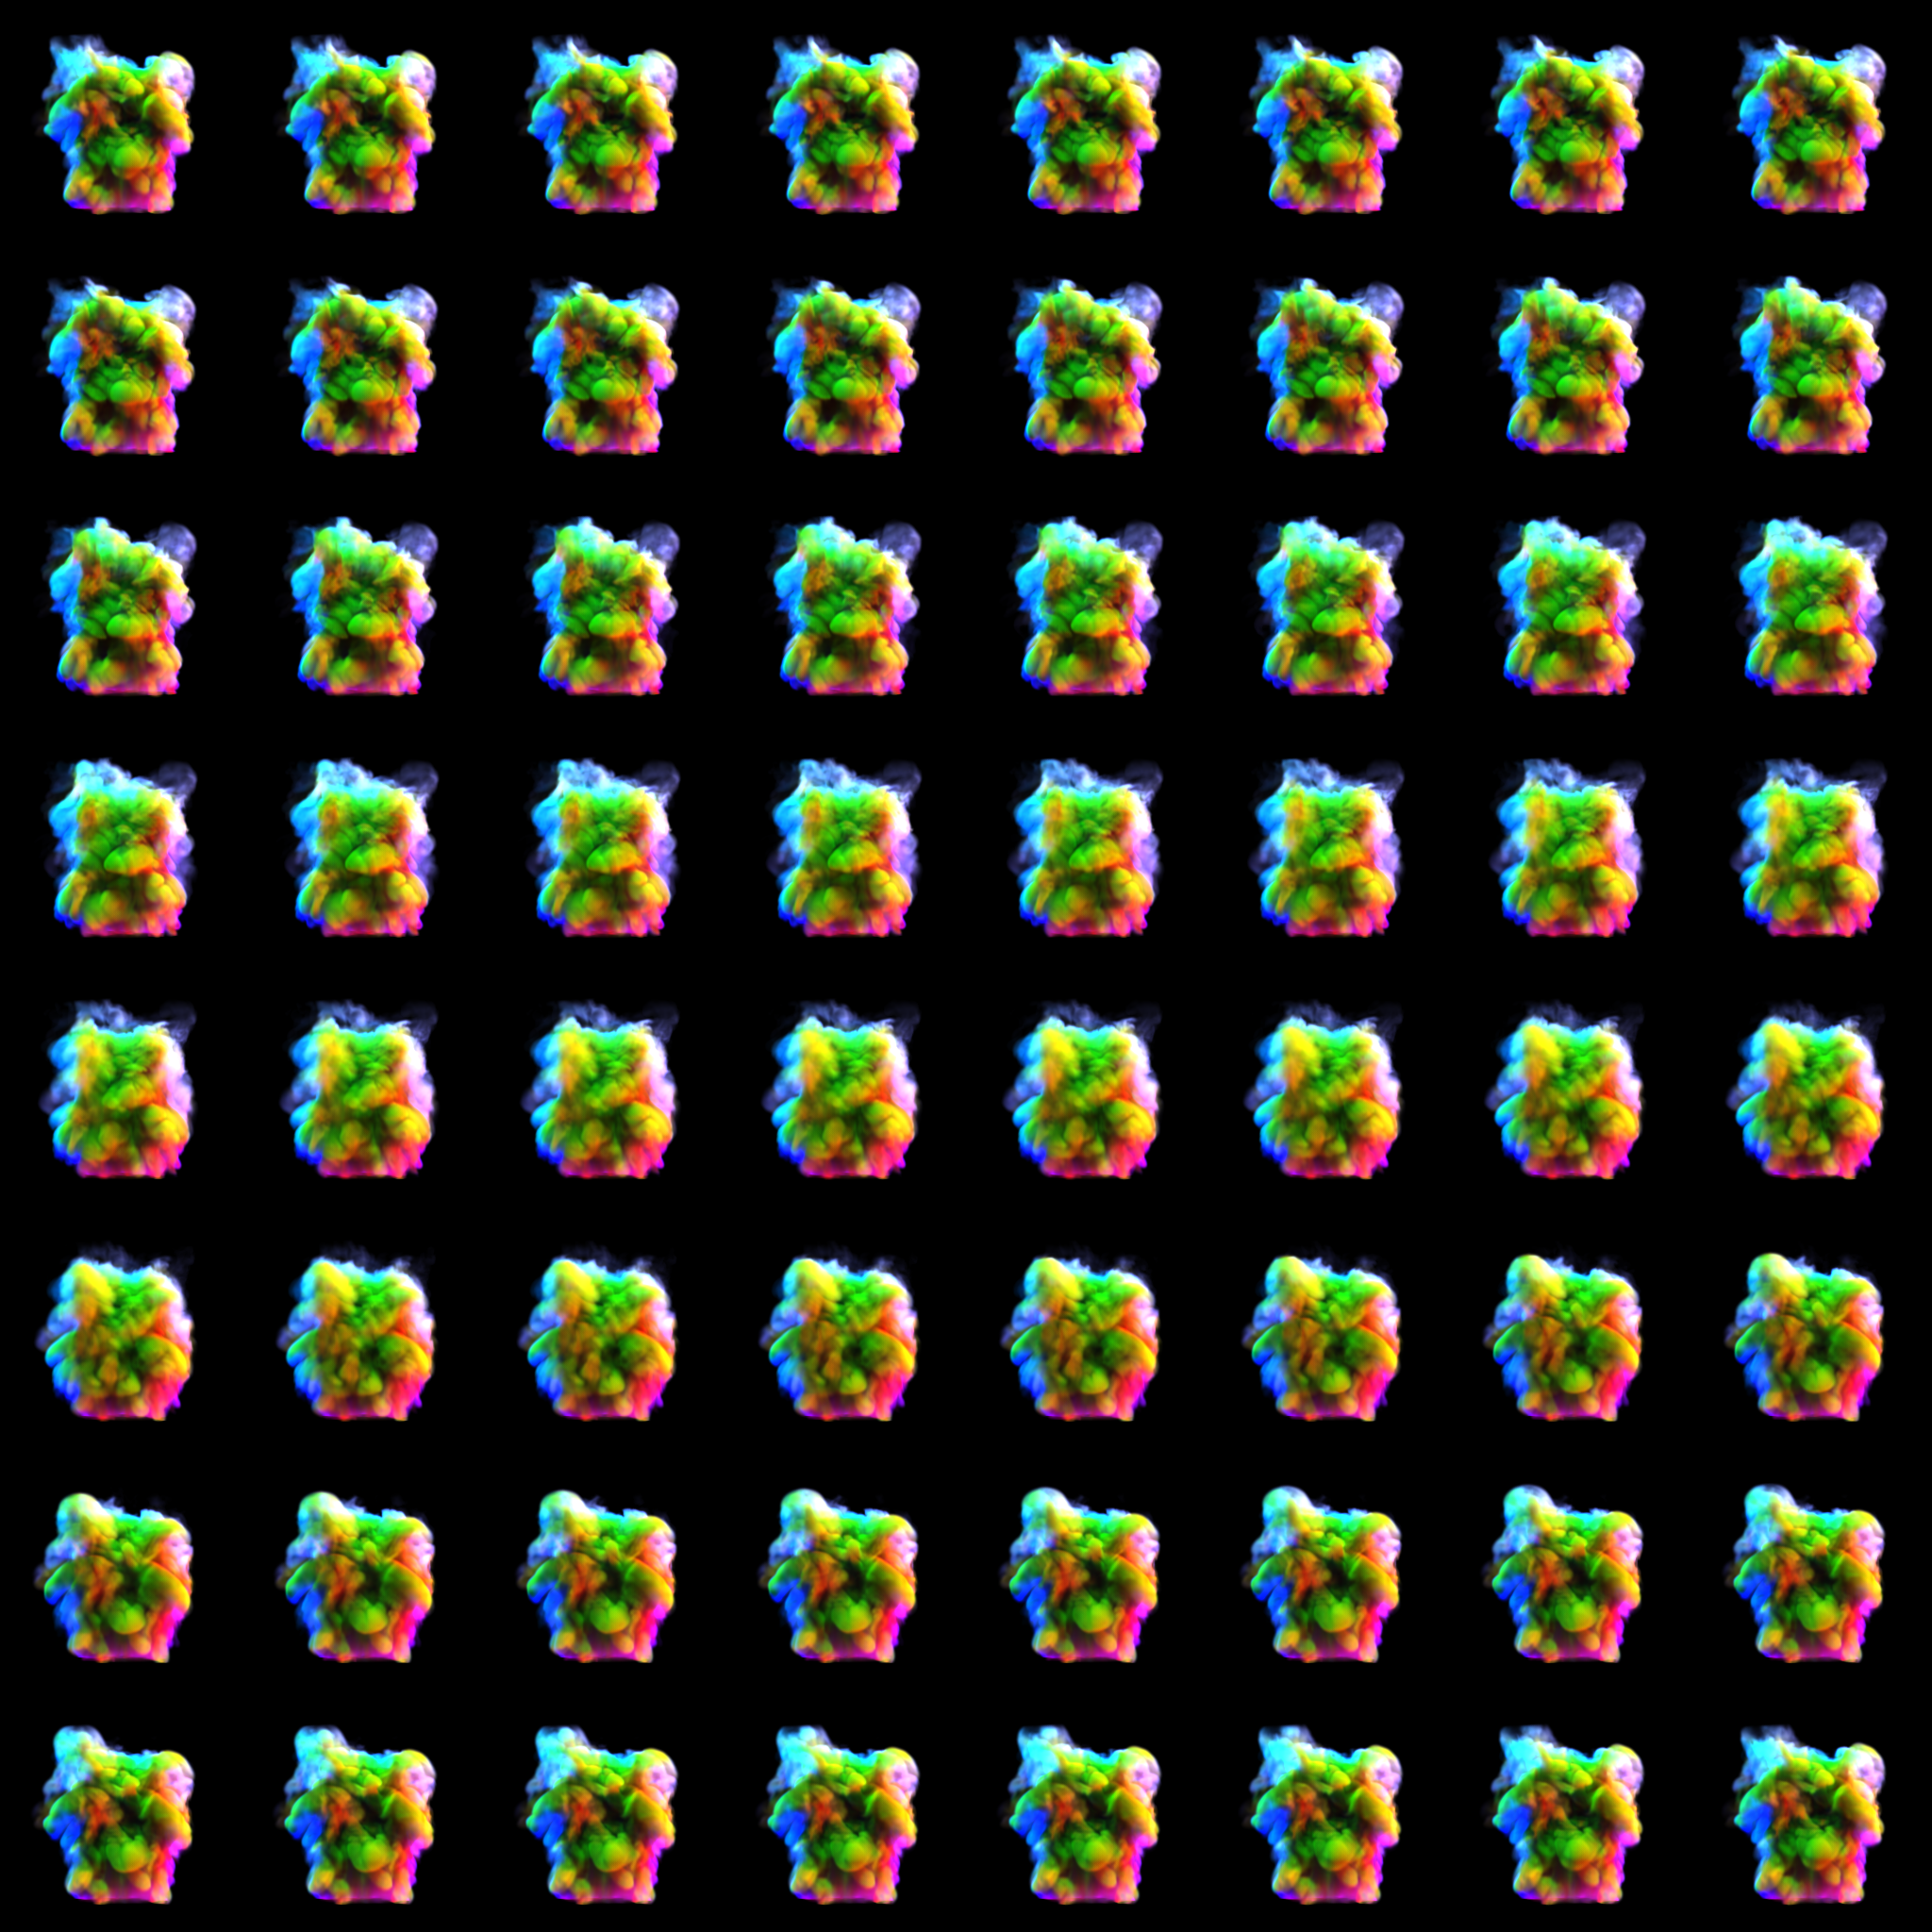
\includegraphics[width=0.49\textwidth]{Grafiken/Implementation/Lightmaps/smokeSim_T1.png}
	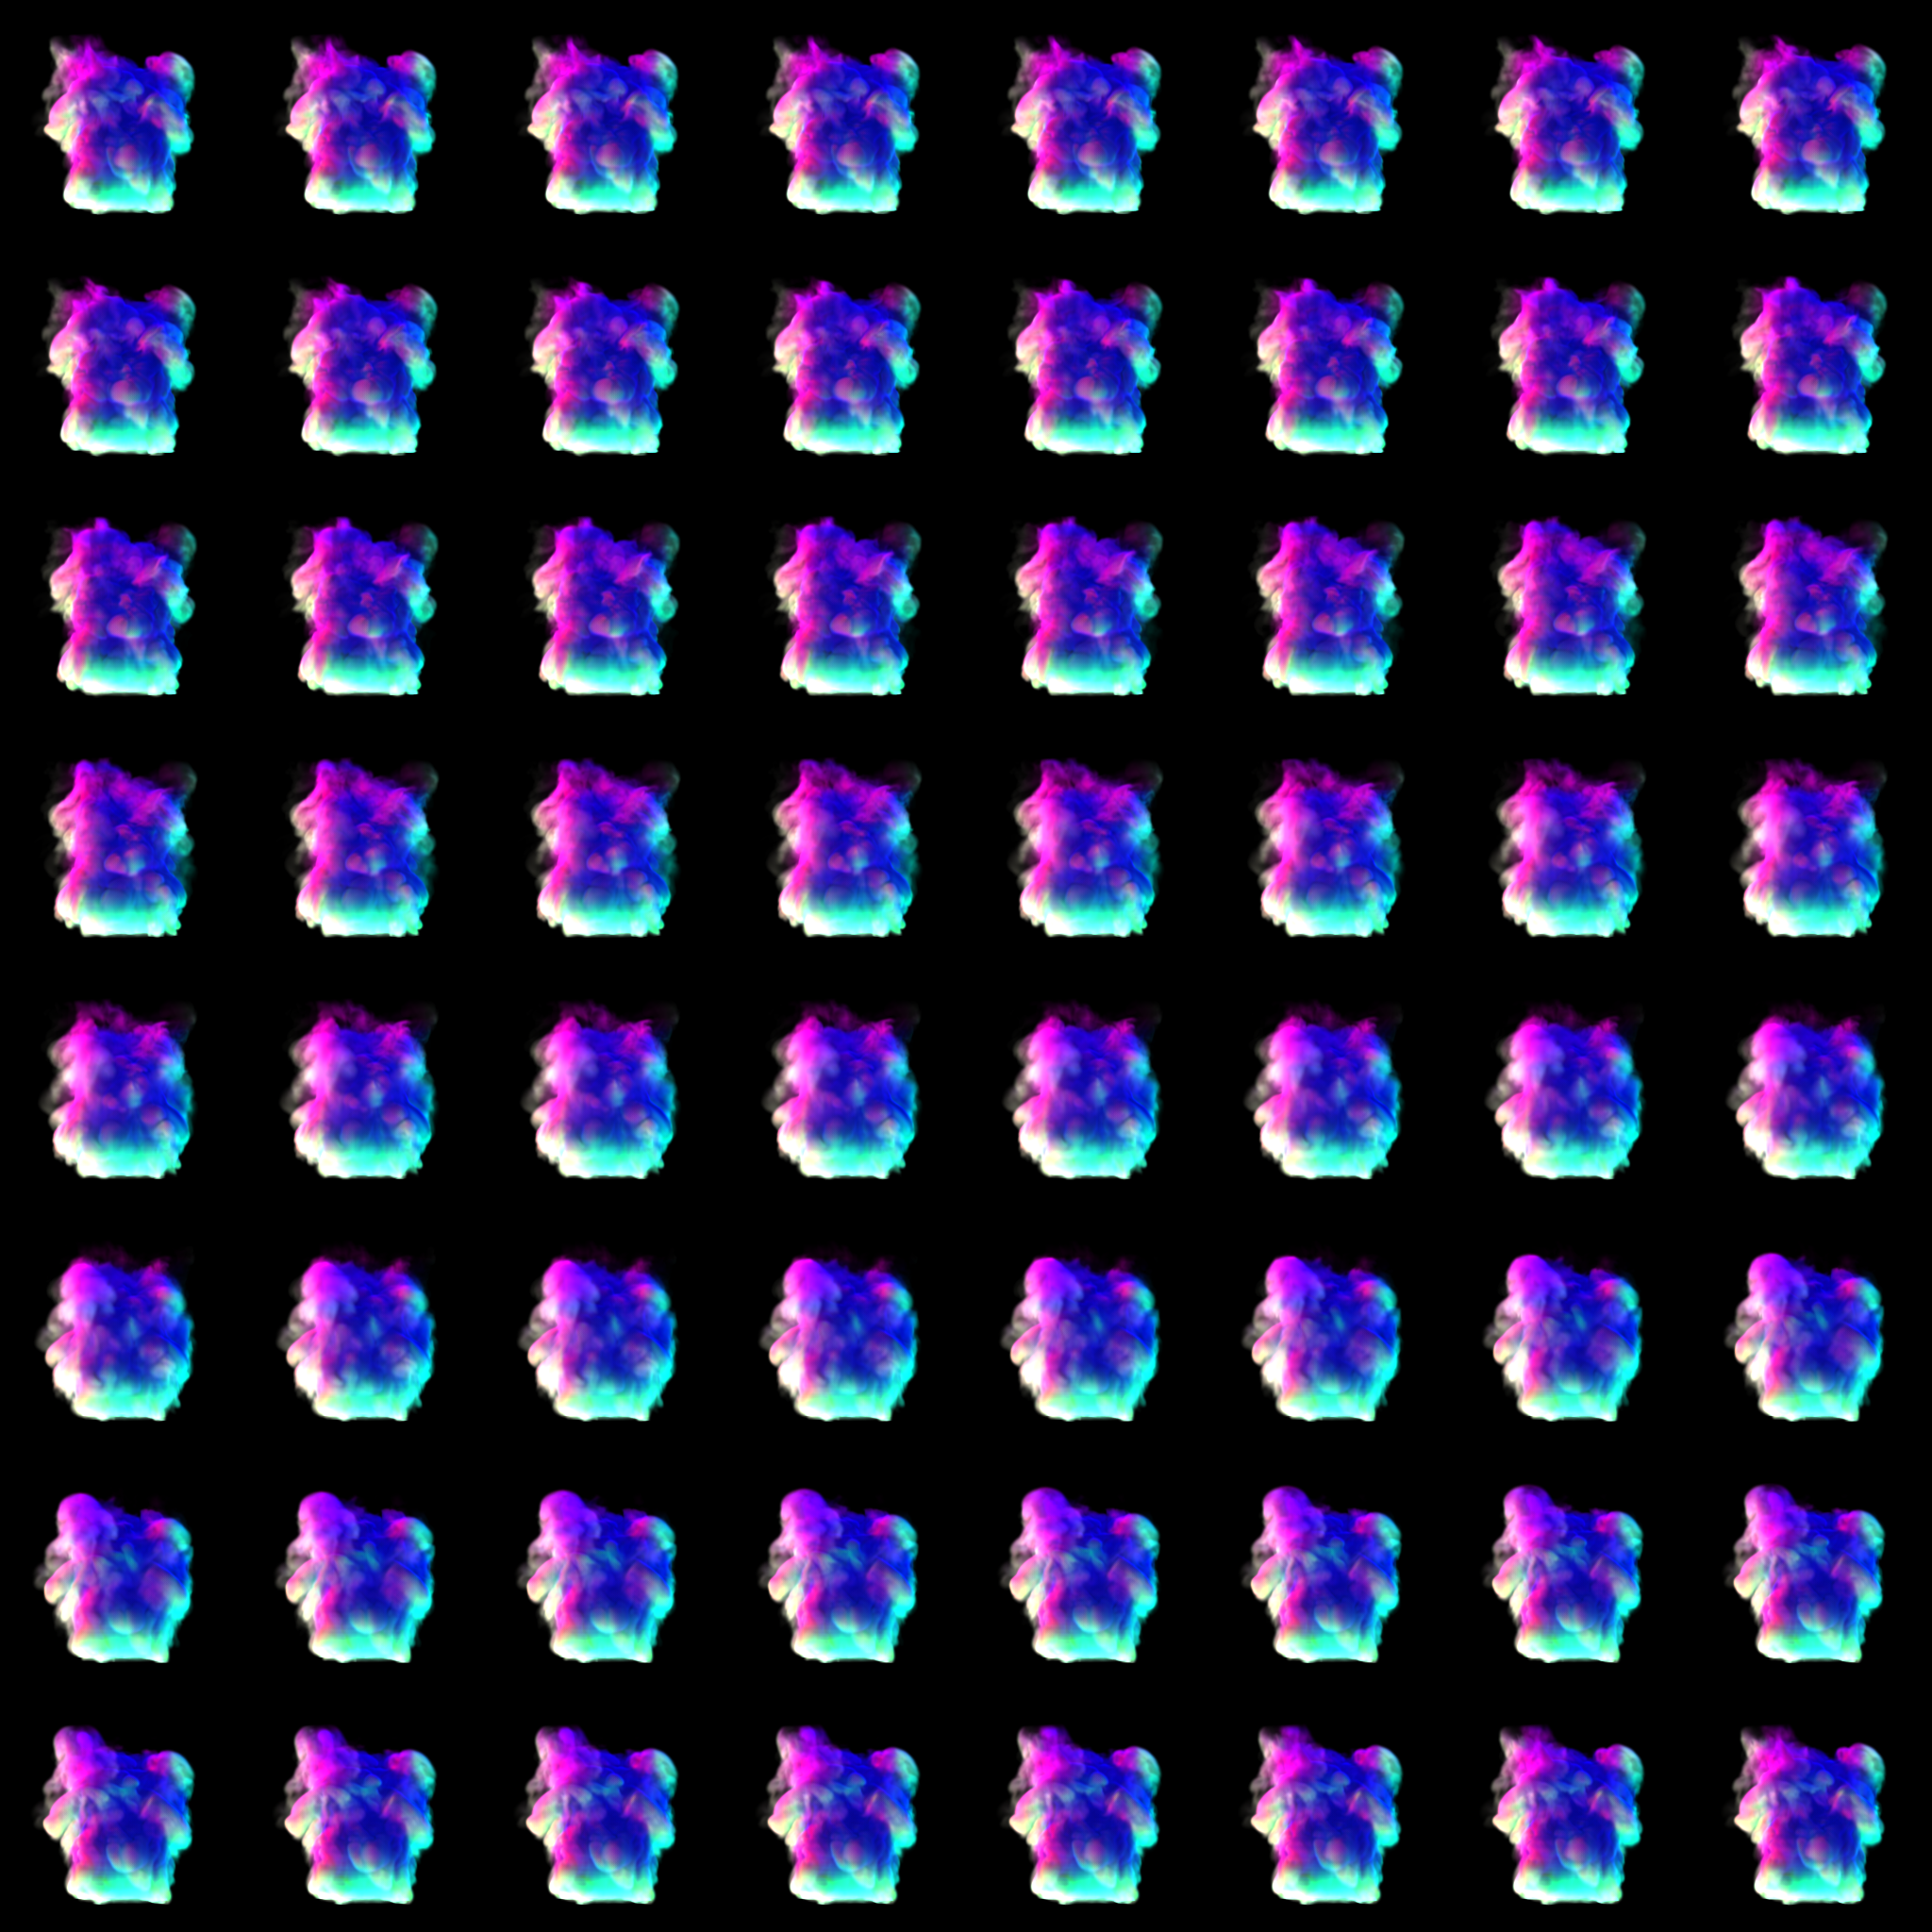
\includegraphics[width=0.49\textwidth]{Grafiken/Implementation/Lightmaps/smokeSim_T2.png}
	\begin{footnotesize}
		\caption{Exportierte Spritesheets aus der Rauchsimulation in Houdini. }
		\label{fig:flipbook}
	\end{footnotesize}
\end{figure}


\subsubsection{Procedural 3D Noise}
TODO




% In den beiden Texturen fehlen nun noch die Beleuchtung aus den Richtungen von Vorne und von Hinten. Diese werden allerdings im Shader
% berechnet, anstatt sie in die Textur zu backen. Aus den verschiedenen Lightmaps kann daraufhin basierend auf der Richtung des Lichteinfalls
% auf die Textur relativ günstig und performant eine korrekte Beleuchtung des Rauchs generiert werden.



% \newpage
% \textcolor{red}{\textbf{TODO:}} \newline
% POM: \newline
% - Alle Steps beschreiben\newline
% - Grafiken einfügen\newline

% RAYM: \newline
% - Volumetextures generieren / downloaden\newline
% - Vorgehen beschreiben\newline
% - Grafiken \newline

% % Raymarching: Volumetextures erstellen.
% Diese werden mithilfe von prozedural generierten Noisetexturen erzeugt.
% Daher basiert der zweite Ansatz auf dreidimensionalen Volumentexturen, welche mithilfe von Raymarching gesampled werden.


\subsection{Shader}
Für das Rendering der Partikel werden zwei Shader entwickelt. Diese basieren auf Parallax Occlusion Mapping und auf einem Raymarchingalgorithmus
durch eine Volumentextur. Für POM wird Unitys Shader Graph verwendet. Shader Graph ist, genau wie Unitys VFX Graph, ein Node-Editor um
schnell und übersichtlich Shader zu entwickeln. Hier besteht die Möglichkeit auch eigene Funktionen in Nodes
zu verpacken und somit auf visuelle Art und Weise zu entwickeln. Dies macht vorallem das Debugging einfacher und erlaubt das schnelle Prototyping von Ideen,
da einiges an Boilerplate-Code erspart wird.


\subsubsection{Parallax Occlusion Mapping}

Um die einzelnen Frames aus den Texture Sheets als Animation darstellen zu können, wird ein Flipbook-Node\footnote{\url{https://docs.unity3d.com/Packages/com.unity.shadergraph@12.0/manual/Flipbook-Node.html}}
verwendet. Dieser manipuliert die UV-Koordinaten mithilfe der Information über Zeilen und Spalten des Texture Sheets,
sodass die Koordinaten eines jeden Frames abhängig von der Zeit ausgegeben werden.
Somit lässt sich auch die Framerate anpassen, mit der die Animation abgespielt werden soll.

Diese UV-Koordinaten werden nun in einen Parallax Occlusion Mapping-Node weitergegeben, hier wird ebenfalls der Node von Unity\footnote{\url{https://docs.unity3d.com/Packages/com.unity.shadergraph@12.0/manual/Parallax-Occlusion-Mapping-Node.html}}
benutzt. Dieser berechnet, basierend auf den übergebenen UV-Koordinaten des Flipbook-Players, sowie einer Heightmap und dem Blickwinkel die anzuzeigenden Texturkoordinaten.
Es lassen sich außerdem die Anzahl der Schritte mit denen die Heightmap abgetastet werden soll, sowie die Amplitude des Offsets festlegen.
Für die Implementierung des Rauchs wurde die Schrittanzahl auf 150 und die Amplitude auf 1 bis 3.5 gesetzt. Diese Werte haben sich durch ausprobieren ergeben.
Eine höhere Amplitude verzerrt den Rauch so stark, sodass die in \autoref{sec:3.3.4} beschriebenen Artefakte auftreten.

\textcolor{red}{>>SCREENSHOT VON ZU STARK VERZERRTEM RAUCH<<}

Da die Beleuchtung des Rauchs zuvor in Houdini durchsimuliert und abgespeichert wurde muss im Shader nun eine Logik implementiert werden, welche jeweils die richtige Beleuchtung,
abhängig von der Lichtrichtung anzeigt. Die durch den Flipbook- und POM-Node modifizierten UV-Koordinaten werden nun auf das Texture-Sheet abgebildet und somit die Animation durchlaufen.
Da durch das Parallax Mapping die Koordinaten je nach Amplitude unterschiedlich stark verzerrt werden, muss der Rauch maskiert werden um das Fragmente, die am Rand erscheinen auszublenden.
Mit der maskierten Animation kann dann unter einbeziehen des Main Lights (in Unity definiert als die Sonne, also ein directional light). Directional Lights haben keine Position,
lediglich eine Richtung in die sie zeigen. Mithilfe dieser Richtung kann die korrekte Lightmap des Rauchs ausgewählt werden oder je nach Richtung des Lichts
zwischen verschiedenen Maps interpoliert werden. Im Prinzip wird also für jede Achse des Lichts abgefragt, in welche Richtung das Licht zeigt und der entsprechende Farbchannel
der Rauchtextur zurückgegeben.

\vspace{.6cm}
\begin{lstlisting}[language={[Sharp]C}, label={lst:lightMapLogik}, caption={Logik zur Auswahl der richtigen Lightmap am Beispiel der X-Richtung des Lichts},captionpos=b, frame=single]
if(direction.X > 0){
  return smokeLightmap_T1.R; 
}
else {
  return smokeLightmap_T2.R; //Licht von links
}

\end{lstlisting}


\subsubsection{Raymarcher}

Da Feuer und Rauch volumetrische Effekte ohne feste Oberfläche sind, lassen sich diese nicht wirklich durch Geometrie abbilden. Die Idee ist also ein
Volumen zu erzeugen und Strahlen durch dieses Volumen zu schicken, welches in festen Abständen das Volumen abtastet um daraus Informationen zu erhalten.
Hierbei wird das Licht, welches ebenfalls in dieses transluzente Volumen eindringt und absorbiert oder gebrochen wird, an jedem Samplepunkt berechnet.

Die Texturen werden daher wie in \textbf{\autoref{sec:4.1}} beschrieben durch generiertes Rauschen erzeugt.
% Um die notwendige Rechenleistung zu reduzieren, wird auch das generierte Rauschen in Texturen gebacken.  



\subsection{Partikelsystem}
Um die Partikelsysteme umzusetzen wird der relativ junge, von Unity entwickelte Editor 'Visual Effects Graph'
(kurz: VFX Graph) verwendet. VFX Graph ist ein nodesbasierter Editor, um schnell
dynamische und komplexe Partikelsysteme zu erzeugen\footnote{\url{https://unity.com/de/visual-effect-graph}}.
Im Gegensatz zum älteren Shuriken-Partikelsystem von Unity werden die Partikel hier auf der GPU
simuliert, wodurch das System deutlich an Performance gewinnt und ein mehr Partikel zeichnen kann.
Shuriken nimmt die Berechnungen im Gegensatz zum VFX Graph auf der CPU vor\footnote{\url{https://docs.unity3d.com/Manual/ChoosingYourParticleSystem.html}}.
Gerade für VR-Anwendungen bietet sich also dieses neue System an.
VFX-Graph hat jedoch nur sehr begrenzte Möglichkeiten, was Physiksimulationen und Kollisionen der Partikel angeht.
Es muss also ein System erstellt werden, welches trotz der Einschränkungen ein möglichst realistisches
Verhalten der Feuer- und Rauchpartikel gewährleistet.




\newpage
